\chapter{Описание общей архитектуры системы} \label{ch1}

Согласно «Чистой Архитектуре» Роберта Мартина \cite{clean-archecture-book}, основная архитектура системы не должна зависеть от конкретных технологий (а скорее наоборот, технологии должны служить для реализации выбранной архитектуры), поэтому начать проектирование я решил именно с неё. Это позволит сразу определиться с форматом общения приложений между собой, а так же сформировать набор технологий которые позволят реализовать выбранную архитектуру. 

\section{Описание предложенного задания} \label{ch1:sec1}

Руководитель технического отдела сформулировал следующие критерии, которым должна соответствовать разработанная система:

\begin{enumerate}
	\item[1] Для взаимодействия с системой необходим веб-интерфейс, который должен быть адаптирован как для мобильных телефонов, так и для экрана монитора.
	\item[2] Поддерживаться две роли: администратор и обычный пользователь.
	\item[3] Админ создает проекты или архивирует их. На данном этапе для проектов храниться только название. Проекты доступны всем существующим пользователям (в том числе и администратору).
	\item[4] На странице проектов для каждого из них доступны следующие операции: пуск/пауза. 
	\item[5] По нажатию на Пуск начинается отсчет времени. Если он уже был запущен ранее - он продолжается. Одновременно для одного пользователя может идти отсчет только по одному проекту. При активации проекта другой запущенный встает на паузу.
	\item[6] Должен быть экран с статистикой по текущему месяцу. Статистика должна отображаться как по проекту в целом, так и по пользователям отдельно. Пример текущего формата вывода статистики представлен на \firef{fig:general-statistic} и \firef{fig:user-statistic}
\end{enumerate} 

\newpage

\begin{figure}[ht!] 
	\center
	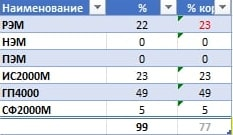
\includegraphics [scale=0.7] {my_folder/images//general_statistics}
	\caption{Пример текущего формата общей статистики} 
	\label{fig:general-statistic}  
\end{figure}

\begin{figure}[ht!] 
	\center
	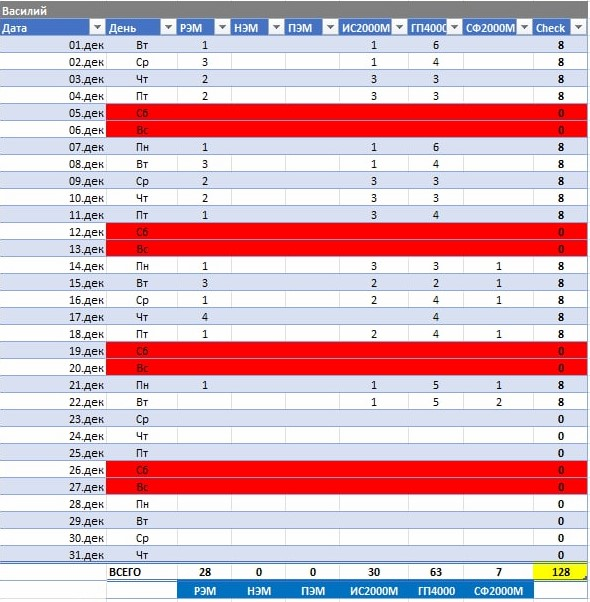
\includegraphics [scale=0.5] {my_folder/images//user_statistics}
	\caption{Пример текущего формата общей статистики} 
	\label{fig:user-statistic}  
\end{figure}


\section{Описание предполагаемой архитектуры} \label{ch1:sec2} 

После анализа предложенного задания и исходя из предметной области, можно сделать вывод, что наиболее предпочтительной архитектурой системы является архитектура 
\textit{«Клиент — сервер»}.

\textbf{Архитектура «Клиент — сервер»} - сборное понятие, состоящее из двух взаимодополняющих компонентов: сервера и клиента.

\textbf{Клиент} — это программа, с которой работает пользователь. Он работает в браузере или с desktop-приложением. В разрабатываемой системе в качестве клиента будет использоваться веб-интерфейс.

\textbf{Сервер} - это компьютер, на котором хранится само приложение. Весь код, вся логика, все дополнительные материалы и справочники. Так же сервер обычно разделяют на две сущности: сервер с основной логикой приложения и сервер с базой данных. 

Простейшая схема клиент-серверной архитектуры представлен на рисунке \firef{fig:client-server-arch}

\begin{figure}[ht!] 
\center
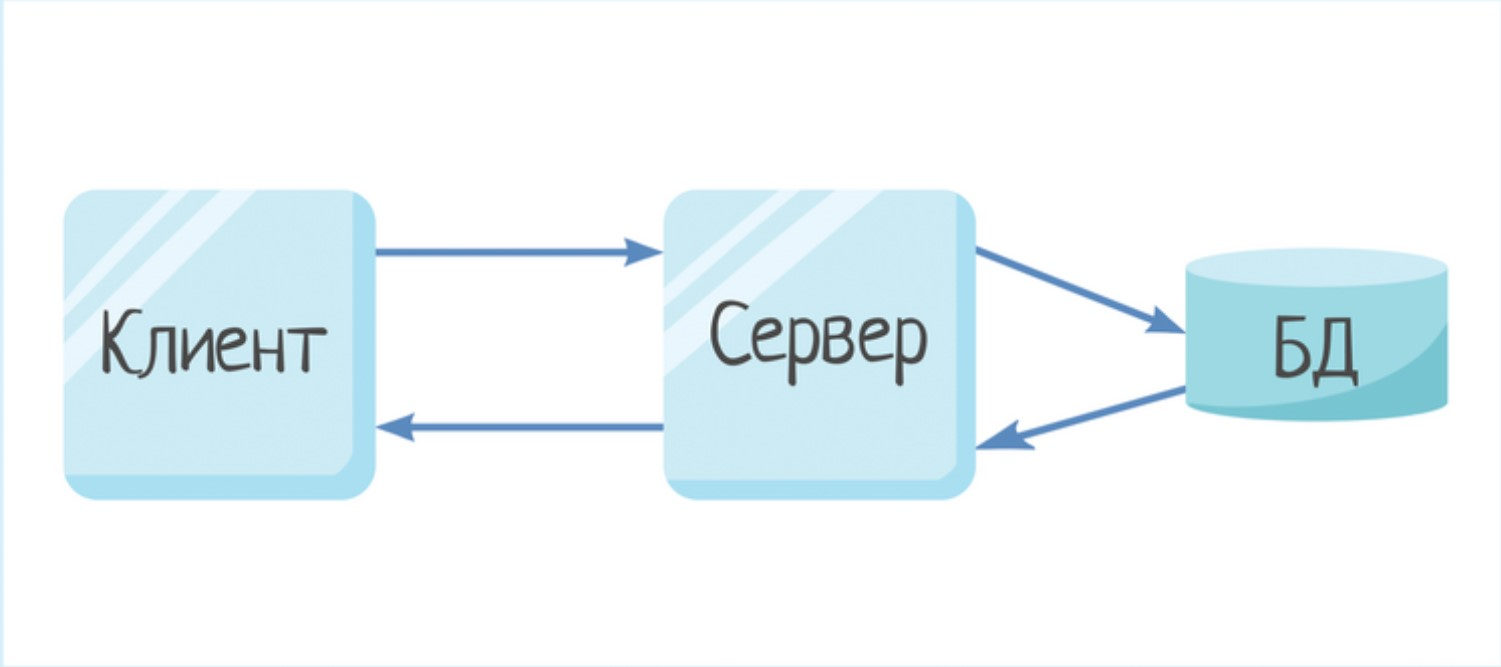
\includegraphics [scale=0.4] {my_folder/images//client-server-arch}
\caption{Архитектура «Клиент — сервер»} 
\label{fig:client-server-arch}  
\end{figure}

Основной причиной использования данной архитектуры является \textbf{централизация обработки входящих запросов}: запросы от всех клиентов обрабатываются и хранятся в одном месте, что позволяет упросить синхронизацию состояний между клиентами. 

В клиент-серверной архитектуре клиент и сервер находятся на разных компьютерах и являются разными приложениями, поэтому им необходим интерфейс для общения. Наиболее популярным на данный момент \textit{RESTful API}. 

\textbf{RESTful API}\cite{restful-api-post} — это интерфейс, используемые двумя компьютерными системами для безопасного обмена информацией через Интернет. Он определяет правила, которым необходимо следовать для связи с другими программными системами. Разработчики внедряют или создают API-интерфейсы, чтобы другие приложения могли программно взаимодействовать с их приложениями. 

Основной концепцией REST является то, что все данные представляются в виде ресурсов , которые хранятся в определенных местах. Клиент связывается с сервером с помощью API, когда ему требуется какой-либо ресурс. 

Основные этапы запроса REST API:
\begin{enumerate}
	\item[1] Клиент отправляет запрос на сервер. Руководствуясь документацией API, клиент форматирует запрос таким образом, чтобы его понимал сервер.
	\item[2] Сервер аутентифицирует клиента и подтверждает, что клиент имеет право сделать этот запрос.
	\item[3] Сервер получает запрос и внутренне обрабатывает его.
	\item[4] Сервер возвращает ответ клиенту. Ответ содержит информацию, которая сообщает клиенту, был ли запрос успешным. Также запрос включает сведения, запрошенные клиентом.
\end{enumerate}

Традиционно, для передачи запросов от клиента к серверу используется протокол передачи гипертекста (\textit{HTTP}). В качестве адреса доступа к ресурсу используется URL. Также, протокол HTTP поддерживает большой набор методов обращения к серверу, наиболее используемые это GET, POST, PUT, DELETE. Метод HTTP сообщает серверу, что ему необходимо сделать с ресурсом. Например, если метод у запроса GET то серверу необходимо вернуть информацию о данном ресурсе, а если DELETE - то удалить данный ресурс. 

После обработки пришедшего запроса сервер должен сформировать ответ. Каждый ответ сервера должен содержать код ответа, по которому клиент понимает результат выполнения запроса. Например, коды 2XX указывают на успешное выполнение, а коды 4XX и 5XX — на ошибки. Также большинство ответов сервера могут содержать тело ответа, в котором храниться ответ сервера, например определенное представление ресурса. 

Так как клиент и сервер должны пересылать представления ресурсов, необходимо выбрать определенный формат этого представления. В качестве такого формата  я выбрал JSON, ввиду его простоты и гибкости. На \firef{fig:json} представлен пример ресурса в формате JSON. 

\begin{figure}[ht!] 
	\center
	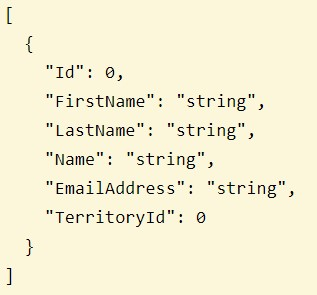
\includegraphics [scale=0.6] {my_folder/images//json}
	\caption{JSON} 
	\label{fig:json}  
\end{figure}

Я выбрал RESTful API как основной интерфейс обращения к серверу в силу следющих его преимуществ: 

\begin{itemize}
	\item Системы, реализующие REST API, могут эффективно масштабироваться благодаря оптимизации взаимодействия между сервером и клиентом по REST.
	\item Веб-службы RESTful поддерживают полное разделение клиента и сервера. Они упрощают и разделяют различные серверные компоненты, чтобы каждая часть могла развиваться независимо. Изменения платформы или технологии в серверном приложении не влияют на клиентское приложение. Возможность разделения функций приложения на уровни еще больше повышает гибкость. Например, разработчики могут вносить изменения в уровень базы данных, не переписывая логику приложения.
	\item REST API не зависит от используемой технологии. Вы можете создавать как клиентские, так и серверные приложения на разных языках программирования, не затрагивая структуру API. Также можно изменить базовую технологию на любой стороне, не влияя на обмен данными.
\end{itemize}


%Формулы могут быть размещены в несколько строк. Чтобы выставить номер формулы напротив средней строки, используйте окружение \verb|multlined| из пакета \verb|mathtools| следующим образом :
%
%\begin{equation} 
%\label{eq:fConcept-order-ch1}
%\begin{multlined}
%(A_1,B_1)\leq (A_2,B_2)\; \Leftrightarrow \\  \Leftrightarrow\; A_1\subseteq A_2\; \Leftrightarrow \\ \Leftrightarrow\; B_2\subseteq B_1. 
%\end{multlined}
%\end{equation}


%Используя команду \verb|\labelcref| из пакета \verb|cleveref|, допустимо следующим образом оформлять ссылку на несколько формул:
%(\labelcref{eq:Pi-ch1,eq:fConcept-order-ch1}).
%
%
%На \firef{fig:spbpu_whitehall-three-photos} приведены три картинки под~общим номером и~названием, но с раздельной нумерацией подрисунков посредством пакета \verb|subcaption|.
%
\begin{figure}[!htbp]
	\adjustbox{minipage=1.3em,valign=t}{\subcaption{}\label{fig:spbpu_whitehall-a}}%
	\begin{subfigure}[t]{\dimexpr.3\linewidth-1.3em\relax}
		\centering
		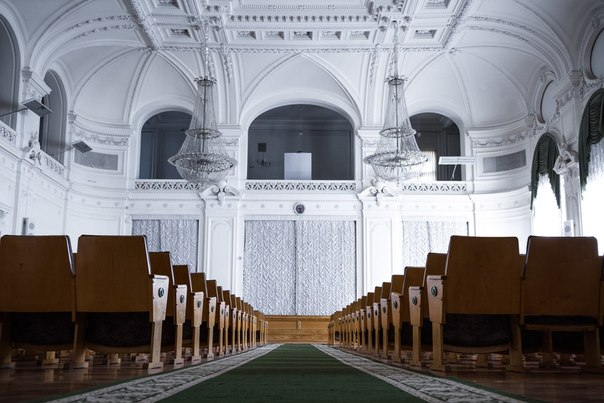
\includegraphics[width=.95\linewidth,valign=t]{my_folder/images//spbpu_whitehall}
	\end{subfigure}
	\hfill %выровнять
	\adjustbox{minipage=1.3em,valign=t}{\subcaption{}\label{fig:spbpu_whitehall-b}}%
	\begin{subfigure}[t]{\dimexpr.3\linewidth-1.3em\relax}
		\centering
		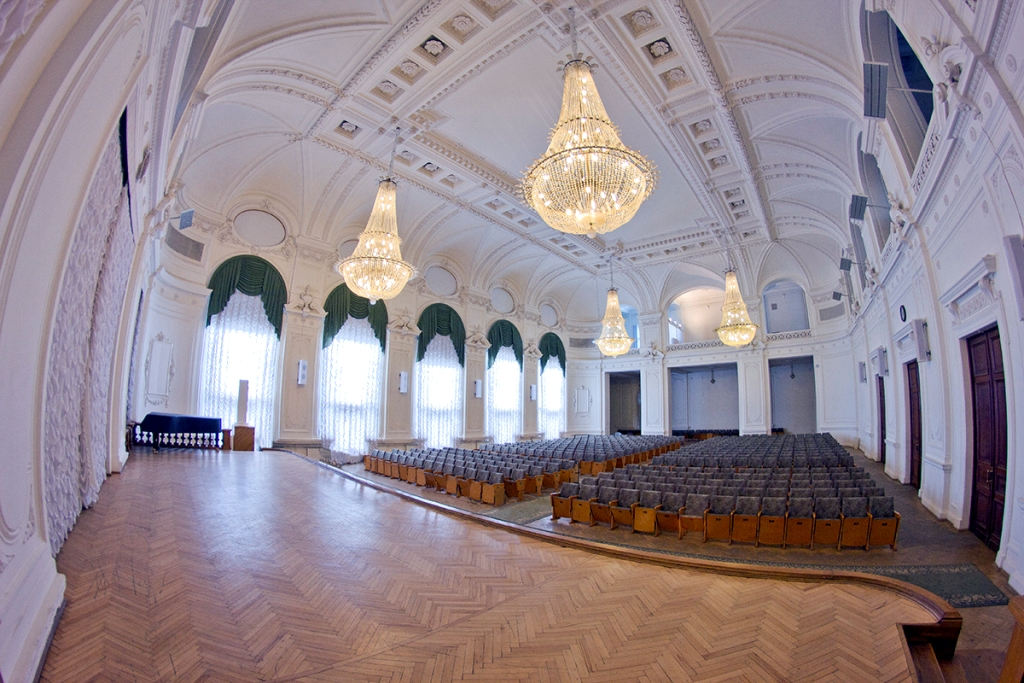
\includegraphics[width=.95\linewidth,valign=t]{my_folder/images//spbpu_whitehall_ligh}
	\end{subfigure}
	\hfill %выровнять
		\adjustbox{minipage=1.3em,valign=t}{\subcaption{}\label{fig:spbpu_whitehall-c}}%
	\begin{subfigure}[t]{\dimexpr.3\linewidth-1.3em\relax}
		\centering
		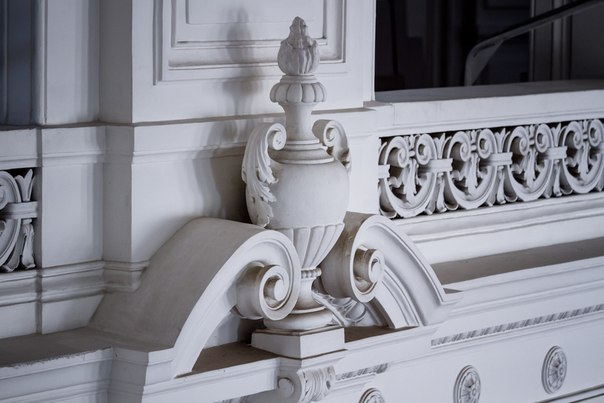
\includegraphics[width=.95\linewidth,valign=t]{my_folder/images//spbpu_whitehall_sculpture}
	\end{subfigure}%
\captionsetup{justification=centering} %центрировать
	\caption{Фотографии Белого зала СПбПУ \cite{spbpu-gallery}, в том числе: {\itshape a} --- со стороны зрителей; {\itshape b} --- со стороны сцены; {\itshape c} --- барельеф}\label{fig:spbpu_whitehall-three-photos}  
\end{figure}

Далее можно ссылаться на три отдельных рисунка: \firef{fig:spbpu_whitehall-a}, \firef{fig:spbpu_whitehall-b} и \firef{fig:spbpu_whitehall-c}. % пример подключения 3х иллюстрации в одном рисунке

%Пример ссылок \cite{Article,Book,Booklet,Conference,Inbook,Incollection,Manual,Mastersthesis,Misc,Phdthesis,Proceedings,Techreport,Unpublished,badiou:briefings}, а также ссылок с указанием страниц, на котором отображены номера страниц  \cite[с.~96]{Naidenova2017} или в виде мультицитаты на несколько источников \cites[с.~96]{Naidenova2017}[с.~46]{Ganter1999}. Часть библиографических записей носит иллюстративный характер и не имеет отношения к реальной литературе. 



%\FloatBarrier % заставить рисунки и другие подвижные (float) элементы остановиться

\section{Резюме} \label{ch1:conclusion}

После анализа поставленной задачи, я решил разбить систему на два приложения: клиент и сервер. В качестве протокола взаимодействия между ними был выбран протокол HTTP, а также в качестве интерфейса обращения к серверному приложению был выбран RESTful API. 

Данная архитектура простая в реализации, а так же позволяет в будущем совершенствовать и масштабировать разработанную систему.
 
\newpage
%Текст выводов по главе \thechapter.

%Кроме названия параграфа <<выводы>> можно использовать (единообразно по всем главам) следующие подходы к именованию последних разделов с результатами по главам:
%\begin{itemize}
%	\item <<выводы по главе N>>, где N --- номер соответствующей главы;
%	\item <<резюме>>;
%	\item <<резюме по главе N>>, где N --- номер соответствующей главы.
%\end{itemize}

%Параграф с изложением выводов по главе \textit{является обязательным}.

%% Вспомогательные команды - Additional commands
%
%\newpage % принудительное начало с новой страницы, использовать только в конце раздела
%\clearpage % осуществляется пакетом <<placeins>> в пределах секций
%\newpage\leavevmode\thispagestyle{empty}\newpage % 100 % начало новой страницы